\section{Uso di Matplotlib per la Visualizzazione dei Dati}

Matplotlib è una libreria potente per la creazione di grafici in Python. Di seguito è riportato un esempio di come realizzare un grafico delle misure sperimentali con barre di errore.

\subsection{Esempio di Grafico}

Consideriamo l'esempio dell'accelerazione di gravità con i seguenti dati:

\[
\begin{array}{c|c}
\text{Tempo (s)} & \text{Distanza (m)} \\
\hline
1.0 & 4.900 \\
2.0 & 19.600 \\
3.0 & 44.100 \\
4.0 & 78.400 \\
5.0 & 122.500 \\
\end{array}
\]

Per mostrare le barre di errore, inseriamo nel codice errori volutamente molto grandi. Si noti inoltre che abbiamo modificato la grandezza dei punti col parametro \textbf{markersize}, la larghezza dei segmenti per le barre con il parametro \textbf{capsize}, e la dimensione del grafico con l'istruzione \textbf{plt.figure(figsize=(12, 9))}.

\begin{lstlisting}[caption={Grafico delle misure sperimentali con barre di errore}]
import numpy as np
import numpy as np
import matplotlib.pyplot as plt

# Dati sperimentali
tempo = np.array([1.0, 2.0, 3.0, 4.0, 5.0])
distanza = np.array([4.900, 19.600, 44.100, 78.400, 122.500])
error_distanza = np.array([1, 2, 3, 1, 4])  # Errori aumentati
error_t2 = np.array([1, 1, 1, 1, 1])

# Configurazione per usare LaTeX in Matplotlib


# Creazione del grafico con dimensioni maggiori e punti più piccoli
plt.figure(figsize=(12, 9))  # Dimensioni della figura
plt.errorbar(tempo**2, distanza, yerr=error_distanza, xerr=error_t2, fmt='o', label='Dati sperimentali', capsize=5, elinewidth=2, markersize=6)
plt.title(r"Misurazione dell'Accelerazione di gravità", fontsize=16)
plt.xlabel(r'Tempo al quadrato (s^2)', fontsize=14)
plt.ylabel(r'Distanza (m)', fontsize=14)
plt.legend()
plt.grid(True)
plt.savefig('grafico_misure.png')  # Salvataggio dell'immagine
#se vuoi scaricare il file da google colab decommenta le righe:
#from google.colab import files
#files.download('grafico_misure.png')
plt.show()



\end{lstlisting}

Nella figura \ref{fig:grafico_misure} è mostrato il grafico risultante.

\begin{figure}[h!]
    \centering
    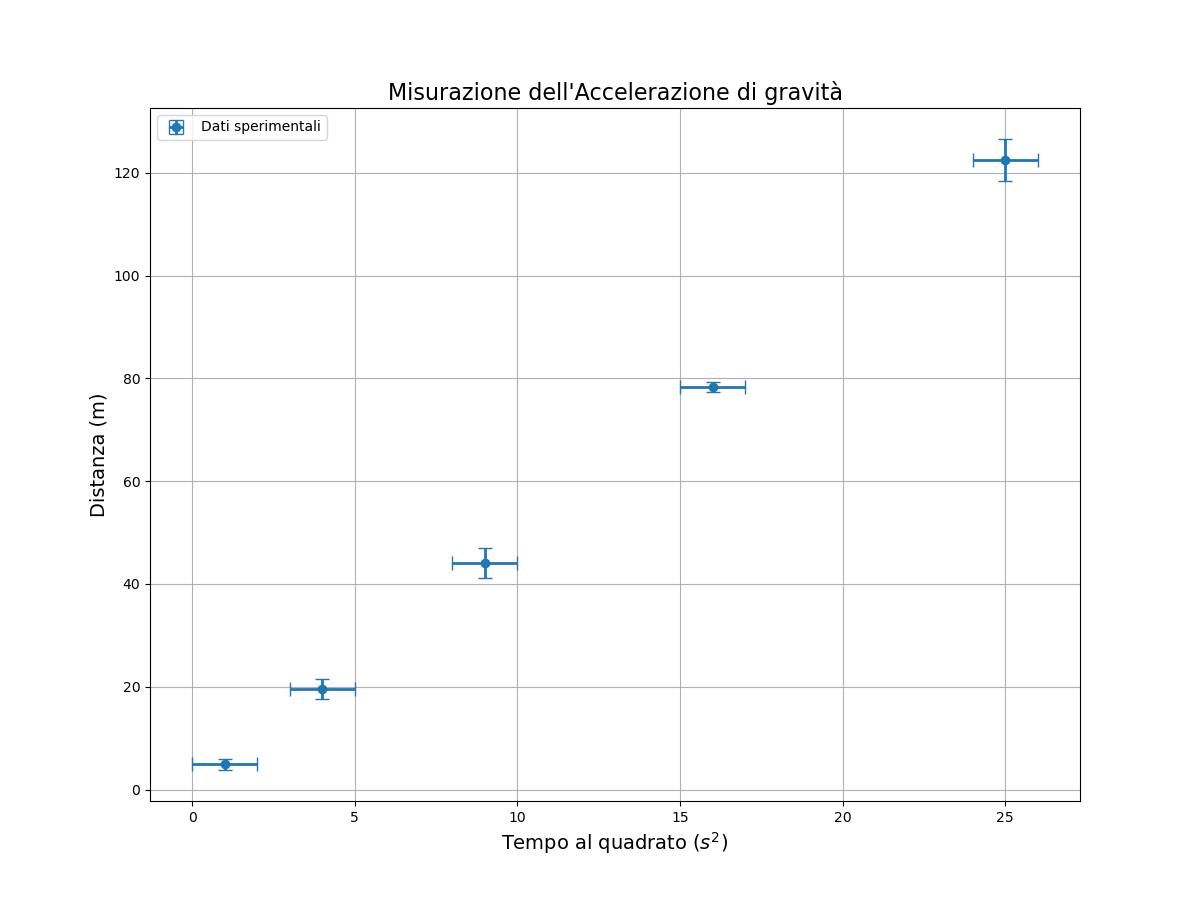
\includegraphics[width=\textwidth]{grafico_misure.png}
    \caption{Grafico delle misure sperimentali con barre di errore.}
    \label{fig:grafico_misure}
\end{figure}


